\documentclass[a4paper,12pt]{article}


\author{\vspace{0.01cm}Marko Gjorgjievski \and Adam Algallaf \and Maximilian Schaefer}
\title{\vspace{-3.4cm}\textbf{Traffic Light Circuit}}
\date{28th June 2020}

\usepackage{fancyhdr}
\usepackage{graphicx}
\usepackage[utf8]{inputenc}	
\usepackage{url}
\usepackage[english]{babel}
\usepackage{hyperref}
\usepackage{wrapfig}
\usepackage{listings}
\usepackage{xcolor}
\usepackage{tikz-timing}
\usepackage{tikz}
\usepackage{makecell}
\usetikzlibrary{arrows,automata}
\lstdefinelanguage{VHDL}{
	morekeywords=[1]{
		BIT,END,OR,ENTITY,IS,PORT,IN,OUT,WITH,
		INOUT,ARCHITECTURE,OF,PROCESS,LIBRARY,
		USE,INTEGER,RANGE,TO,WHEN,ELSE,BEGIN,SELECT,
		AND,SIGNAL,XOR,COMPONENT,NOT,IF,ELSIF,OTHERS,
		THEN,DOWNTO,ALL,INTEGER,GENERIC,CONSTANT,MAP,
		TYPE,SUBTYPE,ARRAY,SLL,SRL,SLA,SRA,ROR,ROL,CASE,
		bit,end,or,entity,is,port,in,out,with,
		inout,architecture,of,process,library,
		use,integer,range,to,when,else,begin,select,
		and,signal,xor,component,not,if,elsif,others,
		then,downto,all,integer,generic,constant,map,
		type,subtype,array,sll,srl,sla,sra,ror,rol,case,
	},   
	morekeywords=[2]{
		STD_LOGIC_VECTOR,STD_LOGIC,IEEE,STD_LOGIC_1164,TO_UNSIGNED,
		NUMERIC_STD,STD_LOGIC_ARITH,STD_LOGIC_UNSIGNED,RISING_EDGE,
		std_logic_vector,std_logic,ieee,std_logic_1164,to_unsigned,
		numeric_std,std_logic_arith,std_logic_unsigned,rising_edge,
	},
	morecomment=[l]--
}
\colorlet{keyword}{blue!100!black!80}
\colorlet{keyword2}{red!80}
\colorlet{comment}{green!60!black}
\lstdefinestyle{vhdl}{
	language     = VHDL,
	basicstyle   = \footnotesize\ttfamily,
	keywordstyle = [1]\color{keyword}\bfseries,   
	keywordstyle = [2]\color{keyword2}\bfseries,
	commentstyle = \color{comment},
	stringstyle = \color{gray}
}
\setcounter{secnumdepth}{2}

\begin{document}
	
	\begin{titlepage}
	\maketitle
			
			
	\begin{center}
	\includegraphics[width=0.4\textheight]{traffic_light.png}
	\cite{Wiki_trafficlight_pic}
	\end{center}


	\begin{figure}[b]
	\centering
	\includegraphics[width=0.3\textheight]{rwu_logo.png}
	\end{figure}
	
	\thispagestyle{fancy}
	\fancyhf{}
	\lfoot{Mentor: Christopher Bonenberger}
	\rfoot{Hochschule Ravensburg-Weingarten\\ Semester: Summer 2020}
	
	
	\end{titlepage}

	\tableofcontents
	\thispagestyle{empty}
	\newpage
	
	\section{Introduction}
	\setcounter{page}{1}
	
	
	Traffic lights are signaling devices that we encounter all the time every day that are used to regulate traffic flow, as given in \cite{Wiki_trafficlight}, it is almost impossible to go anywhere without having to cross a traffic signal.
	
	Without these signaling devices, everyday traffic would not be able to operate as efficiently as it does right now, and it would result in utter chaos on the roads and accidents. We encounter traffic lights daily, yet we rarely stop and question ourselves how do traffic lights function and work. As we almost always take this box with 3 distinct light bulbs tied with a simple circuit for granted, forgetting the crucial yet subtle role it plays in our transportation. 
	
	That is why it sparked the curiosity of my team and that is the reason why we choose to explore and research the traffic light circuit with the intent of making one.
	
	\section{Traffic Light: Type}
	
	As we all know there are numerous types of traffic lights that are used in specific situations on the roads today. Each type is programmed to act according to the road or intersection that it is placed on. As we aimed primarily towards simplicity, we choose to code a traffic light controller circuit which is independent of the placement and stops or allows traffic or pedestrians crossing and with that included, a crossing button which when pressed forces the traffic light to change states and prepare to stop traffic and allowing pedestrians to cross. As a result, we have coded (in VHDL) and simulated a single traffic light controller circuit in ModelSim. The expected behavior of the traffic light is as follows:
	
	\begin{itemize}
	\item To simultaneously stop traffic flow and pedestrians crossing for 30 seconds. (Two red lights for 30 sec.)
	\item Holding traffic for 3 more seconds before allowing \textbf{only} traffic to flow. (Yellow road, red pedestrian for 3 sec.)
	\item Allowing traffic to flow while still holding pedestrians for 27 seconds. (Green road, red pedestrian for 27 sec.)
	\item Preparing to stop the traffic flow in the following 3 seconds.
	(Yellow road, red pedestrian for 3 sec.)
	\item Halting traffic flow and preparing to allow pedestrians to cross which lasts 5 seconds. (Two red lights 5 sec.)
	\item Still holding traffic while allowing pedestrians to cross for 10 seconds. (Red road, green pedestrian for 10 sec. )
	\item Looping the process described above until the simulation reaches the end of run time.
	\item Looping the same process until the crossing button which in turn forces the traffic light to change to the appropriate state.
	
	\footnotetext{``Counter++'' alludes to the incrementation of the counter signal by one or $counter=counter+1$.}
	
		\begin{figure}[h]
			\centering
		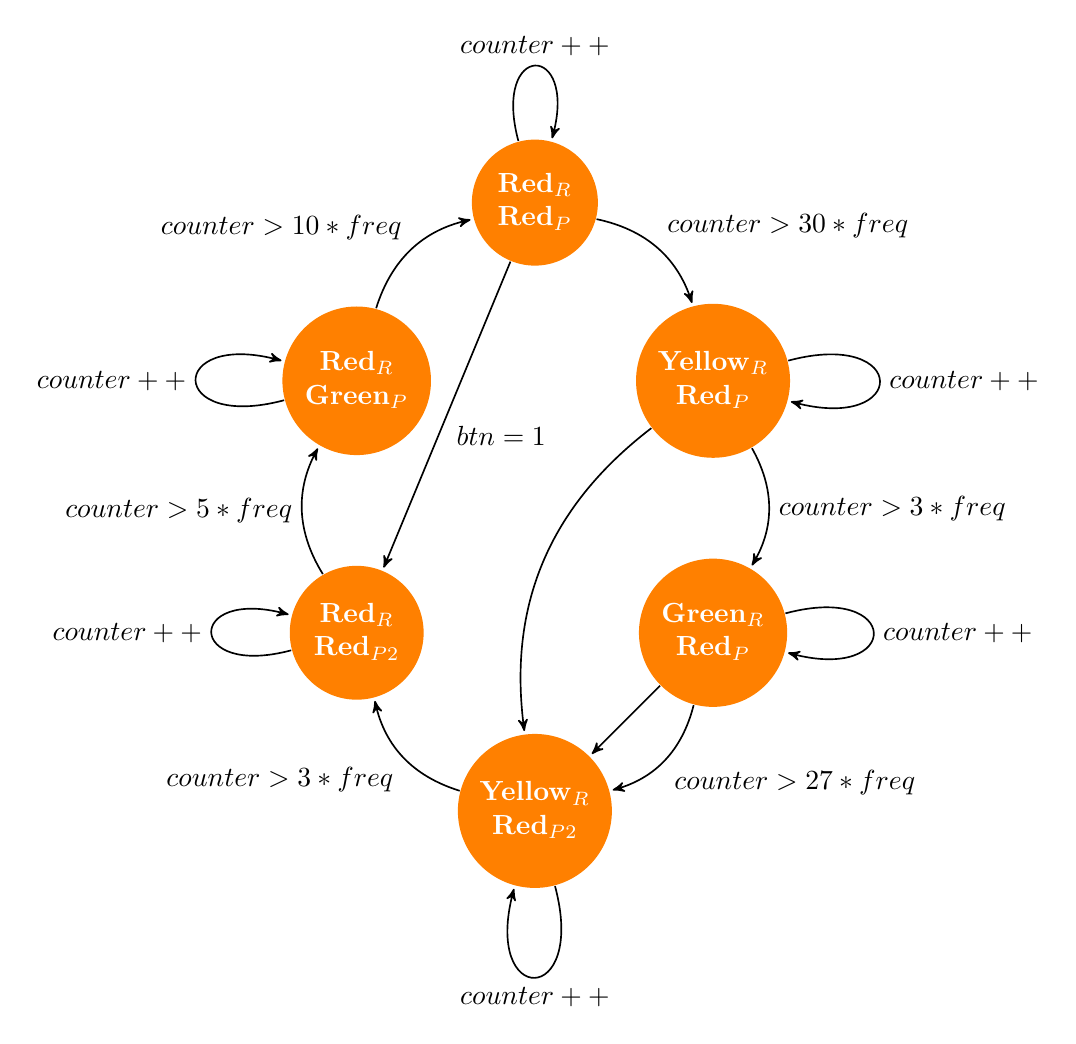
\begin{tikzpicture}[->,>=stealth',shorten >=1pt,auto,node distance=3.2cm,
		semithick]
		\tikzstyle{every state}=[fill=orange,draw=none,text=white]
		
		\node[state] (A)                    {\makecell[c]{$\mathbf{Red}_R$\\$\mathbf{Red}_P$}};
		\node[state] (B) [below right of=A] {\makecell[c]{$\mathbf{Yellow}_R$\\$\mathbf{Red}_P$}};
		\node[state] (C) [below of=B] {\makecell[c]{$\mathbf{Green}_R$\\$\mathbf{Red}_P$}};
		\node[state] (D) [below left of=C] {\makecell[c]{$\mathbf{Yellow}_R$\\$\mathbf{Red}_{P2}$}};
		\node[state] (E) [above left of=D] {\makecell[c]{$\mathbf{Red}_R$\\$\mathbf{Red}_{P2}$}};
		\node[state] (F) [below left of=A] {\makecell[c]{$\mathbf{Red}_R$\\$\mathbf{Green}_P$}};
		
		\path 
		(A) edge [loop above] node {$counter++$} (A)
		edge [bend left] node {$counter > 30*freq$} (B)
		(B) edge [loop right] node {$counter++$} (B)
		edge [bend left]  node {$counter > 3*freq$} (C)
		(C) edge [loop right] node {$counter++$} (C)
		edge [bend left] node {$counter > 27*freq$} (D)
		(D) edge [loop below] node {$counter++$} (D)
		edge [bend left]  node {$counter > 3*freq$} (E)
		(E) edge [loop left]  node {$counter++$} (E)
		edge [bend left]  node {$counter > 5*freq$} (F)
		(F) edge [loop left] node {$counter++$} (F)
		edge [bend left]  node {$counter > 10*freq$} (A)
		(A) edge			  node {$btn=1$} (E)
		(B) edge [bend right]  node {} (D)
		(C) edge 			   node {} (D);
		
		\end{tikzpicture}
		\caption{State flow graph of the traffic light states\label{Stategraph}}
	\end{figure}
		
		
	\end{itemize}
	
	To skip the implementation and see the simulation immediately please refer to section \ref{sim}.
	
	
	\section{VHDL Implementation}
	
	In this section we are going to describe the architecture and behavior of the traffic light circuit written in VHDL.
	
	\subsection{VHDL: Traffic Light Module}
	We begin with the module where the most important processes are present. Inside the file \verb|traffic_light_circuit.vhdl|.
	\begin{figure}[h]
	\begin{lstlisting}[style=vhdl]
library ieee;
use ieee.std_logic_1164.all;
entity traffic_light_circuit is
	generic ( clkFrequency : integer );
	port(
	clk       : in  std_logic;
	btn	  : in  std_logic;    
	rst_n     : in  std_logic;
	Red_R     : out std_logic;
	Yellow_R  : out std_logic;
	Green_R   : out std_logic;
	Red_P	  : out std_logic;
	Green_P	  : out std_logic);
end entity;
	\end{lstlisting}
	\caption{Module: Entity\label{entity}}
	\end{figure}
	
	In the figure \ref{entity} we can see that we have defined inputs for the clocking process that we require for the circuit to work properly.
	We have defined ports for the input clock signal \verb|clk| and a negative reset\footnote{Whenever the reset signal is 0 then the flip-flop is in reset and if the opposite is true (is 1) then it is out of reset.}  \verb|rst_n|. We have also defined the clock frequency in generic so that we can use it later for our counter in real time simulation. And for the outputs we have defined signals for every light respectively.
	\clearpage
	
	\begin{figure}[h]
	\begin{lstlisting}[style=vhdl]
architecture tfcarch of traffic_light_circuit is
type light_t is (RedR_RedP,YellowR_RedP,GreenR_RedP,
YellowR_RedP2,RedR_RedP2,RedR_GreenP);
signal light_s : light_t;
signal counter : integer range 0 to clkFrequency*60;
	\end{lstlisting}
	\caption{Module architecture\label{arch}}
	\end{figure}

	Then inside the architecture of \verb|traffic_light_circuit| we have defined a data type \verb|light_t| which will be used for defining the states in which the circuit enters for displaying the different lights. The signal \verb|light_s| is defined as type \verb|light_t| and will be used as a selector signal in the MUX\footnote{Multiplexer} which is used to change the states.
	
	The \verb|counter| signal with the defined value range will be used for transitioning into different states after a specified amount of time.
	
	\begin{figure}[h]
	\begin{lstlisting}[style=vhdl]
begin
	process (clk) is
begin 
	if(rst_n = '0') then
	light_s   <= RedR_RedP;
	counter   <= 0;
	Red_R     <='1';
	Yellow_R  <='0';
	Green_R   <='0';
	Red_P	  <='1';
	Green_P   <='0';
elsif rising_edge(clk) then
	counter <= counter + 1;
	case light_s is
	\end{lstlisting}
	\caption{Model architecture: Process\label{archproc}}
	\end{figure}

	After the \verb|clk| signal changes the process initiates, first checking if its in active reset and if that condition is met it assigns the initial state \verb|Red_RedP| to the selector signal \verb|light_s|, as well as resetting the \verb|counter| and assigning values to the outputs according to the state.
	
	If the flip-flop is not in active reset, it then checks for the rising edge of the clock and if that condition is met the \verb|counter| increments and we enter the leftmost defined or initial state.
	
	This flip-flop is widely known as an asynchronous active low as cited by \cite{VHDL-Wizz}. 
	\clearpage
	
	\begin{figure}[h]
	\begin{lstlisting}[style=vhdl]
when YellowR_RedP =>
	Red_R     <='0';
	Yellow_R  <='1';
	Green_R   <='0';
	Red_P	  <='1';
	Green_P   <='0';
	if rising_edge(btn) then
		counter <= 0;
		light_s <= YellowR_RedP2;
	end if;
	if(counter >= clkFrequency *3 - 1) then
		counter <= 0;
		light_s <= GreenR_RedP;
	end if;
	\end{lstlisting}
	\caption{Architecture: Sample State \label{archstate}}
	\end{figure}

	In the figure \ref{archstate}, the \verb|light_s| signal is set to \verb|YellowR_RedP| and as we mentioned previously the outputs change in accordance with the current state. After that is finished, it checks for a button press by registering a rising edge from the \verb|btn| signal. If a rising edge is registered then the counter resets and \verb|light_s| changes state so it can allow pedestrians to cross. If not, the counter continues to increment (\ref{archproc}) until it reaches its time threshold (which is dependent on the clock period and frequency and state that it is in, in this case for the yellow it would last 3 seconds in real-time simulation), then it resets and \verb|light_s| changes to the next predefined state.
	
	All the other states are defined in a similar fashion, to see the rest of the architecture please refer to the \verb|traffic_light_circuit.vhdl| file.
	\clearpage
	\subsection{VHDL: Test bench}
	
	Now we need to write a test bench where we can test our complete module in a real time simulation. We will call that test bench \verb|traffic_light_circuit_tb.vhdl|.
	
	\begin{figure}[h]
	\begin{lstlisting}[style=vhdl]
library ieee;
use ieee.std_logic_1164.all;
use ieee.numeric_std.all;
entity traffic_light_circuit_tb is
end entity;
architecture simulation of traffic_light_circuit_tb is
constant clkFrequency: integer := 100;
constant clkPeriod : time   := 1000 ms / clkFrequency;
signal clk      : std_logic := '1';
signal rst_n    : std_logic := '0';
signal btn	: std_logic := '0';
signal Red_R    : std_logic;
signal Yellow_R : std_logic; 
signal Green_R  : std_logic;
signal Red_P	: std_logic;
signal Green_P  : std_logic; 
	\end{lstlisting}
	\caption{Test bench architecture: Signals\label{tb_archsign}}
	\end{figure}

	In the test bench file we define the previously mentioned signals so that we can port them over to the corresponding input and output ports on the traffic light module. We also define the clock period and frequency constants which \textbf{are of utmost importance} for the real-time simulation as the clock and counter signal depend on them.
	
	\begin{figure}[h]
	\begin{lstlisting}[style=vhdl]
tfc_test : entity work.traffic_light_circuit(tfcarch)
generic map (clkFrequency => clkFrequency)
port map (
clk      => clk,
rst_n    => rst_n,
btn      => btn,
Red_R    => Red_R,
Yellow_R => Yellow_R,
Green_R  => Green_R,
Red_P    => Red_P,
Green_P  => Green_P );
	\end{lstlisting}
	\caption{Test bench architecture: Ports\label{tb_archports}}
	\end{figure}

	This is where we declare an instance for our module and where we port the signals.
	
	\begin{figure}[h]
	\begin{lstlisting}[style=vhdl]
	clk <= not clk after clkPeriod / 2;
	process is
	begin
	wait until rising_edge(clk);
	wait until rising_edge(clk);
	rst_n <= '1';
	btn <= not btn after 14000 ms;
	wait until rising_edge(btn);
	btn <= not btn after 2000 ms;
	wait;
	end process;
	end architecture;
	\end{lstlisting}
	\caption{Test bench architecture: Process\label{tb_archproc}}
	\end{figure}
	
	The first statement is a concurrent one so the sensitivity list is on the right. After that, the moment when 2 rising edges are registered the flip-flop comes out of reset and the process begins according to \cite{VHDL-Renerta}. The moment the \verb|btn| has a rising edge (in this case after 14 seconds) then the pedestrian traffic light outputs begin to change as well. After 2 seconds the signal returns to 0 and simulation continues as usual.
	
	\section{Simulation\label{sim}}
	
	After we compile the module and the test bench we simulate the test bench to see if our traffic light circuit is working as intended. The signals in the simulation:
	
	\begin{figure}[h]%[!htb]
		\centering
		\begin{tikztimingtable}[%
			timing/dslope=0.01,	% slope from 0 to 1 or vice versa
			timing/.style={x=1ex,y=1ex},	% basic tik size
			x=1ex,	
			timing/rowdist=2.5ex,
			timing/name/.style={font=\sffamily\scriptsize}
			]
			$\mathbf{btn}$        	& 2.5L 0.33H 10.2L 10.2L 10.2L 8.1L\\
			$\mathbf{Red}_R$        & 2.5H 0.833H 1.66H 5H 0.5L 4.5L 0.5L 0.833H 1.66H 5H 0.5L 4.5L 0.5L 0.833H 1.66H 5H 0.5L 4.5L 0.5L\\
			$\mathbf{Yellow}_R$     & 2.5L 0.833L 1.66L 5L 0.5H 4.5L 0.5H 0.833L 1.66L 5L 0.5H 4.5L 0.5H 0.833L 1.66L 5L 0.5H 4.5L 0.5H\\
			$\mathbf{Green}_R$      & 2.5L 0.833L 1.66L 5L 0.5L 4.5H 0.5L 0.833L 1.66L 5L 0.5L 4.5H 0.5L 0.833L 1.66L 5L 0.5L 4.5H 0.5L\\
			$\mathbf{Red}_P$        & 2.5H 0.833H 1.66L 5H 0.5H 4.5H 0.5H 0.833H 1.66L 5H 0.5H 4.5H 0.5H 0.833H 1.66L 5H 0.5H 4.5H 0.5H\\
			$\mathbf{Green}_P$      & 2.5L 0.833L 1.66H 5L 0.5L 4.5L 0.5L 0.833L 1.66H 5L 0.5L 4.5L 0.5L 0.833L 1.66H 5L 0.5L 4.5L 0.5L\\
		\end{tikztimingtable}\caption{Signals in simulation\label{signalsim}}
		
	\end{figure}

	After running a 5 minute simulation we can see that our traffic light circuit is working as we intended it to, where the time difference between the states are correct and the light signals in each state are changed accordingly.
	
	\section{Final Words}
	
	Tackling this project has been an interesting experience as me and my team throughout the ordeal have learned a great deal about \LaTeX{}, VHDL and ModelSim simulations. We have come to appreciate more the smaller digital circuits that also have their own part in society as well as better understanding them.
	\newline
	The members of our team are: Marko Gjorgjievski, Adam Yousif Algallaf and Maximilian Schaefer.
	\newline
	\newline
	Special thanks to Professor Bonenberger for his lectures and introducing digital circuits to us.
	
	\listoffigures
		
	\begin{thebibliography}{1}
	\bibitem{VHDL-Wizz}
	VHDL-Wizz:
	\url{https://vhdlwhiz.com/} Date of access: 17.06.20
	\bibitem{VHDL-Renerta}
	VHDL-Renerta:
	\url{http://vhdl.renerta.com/} Date of access: 21.06.20
	\bibitem{Wiki_trafficlight}
	Traffic light info:
	\url{https://en.wikipedia.org/wiki/Traffic_light} 
	\bibitem{Wiki_trafficlight_pic}
	Traffic light picture:``Traffic lights display green to indicate "go ahead".''
	\url{https://en.wikipedia.org/wiki/Green-light#/media/File:LED_traffic_light.jpg} Date of access: 15.06.20
	\bibitem{LaTeX-Tutorial}
 	\url{https://www.youtube.com/playlist?list=PL-p5XmQHB_JSQvW8_mhBdcwEyxdVX0c1T} Date of access: 22.06.20
 	\bibitem{VHDL-Tutorial}
 	\url{https://www.youtube.com/watch?v=h4ZXge1BE80&list=PLIbRYKjjYOPkhpxnkQ0fwTXnmgsiCMcVV} Date of access: 17.06.20
 	
 \end{thebibliography}
	
\end{document}